\section{Aufbau}
\label{sec:Aufbau}

Im ersten Versuchsteil im elektrischen Feld wird eine Schaltung gemäß Abbildung \ref{fig:Aufbau-E1} aufgebaut. Die Versorgungsspannung entspricht der Beschleunigungsspannung $U_.B$. An die Ablenkplatten wird eine variable Ablenkspannung $U_.d$ angelegt, welche an dem Voltmeter abgelesen werden kann. Jeweils eine der Platten der Ablenksysteme wird geerdet, wobei darauf geachtet wird, dass Kurzschlüsse vermieden werden.

\begin{figure}
\centering
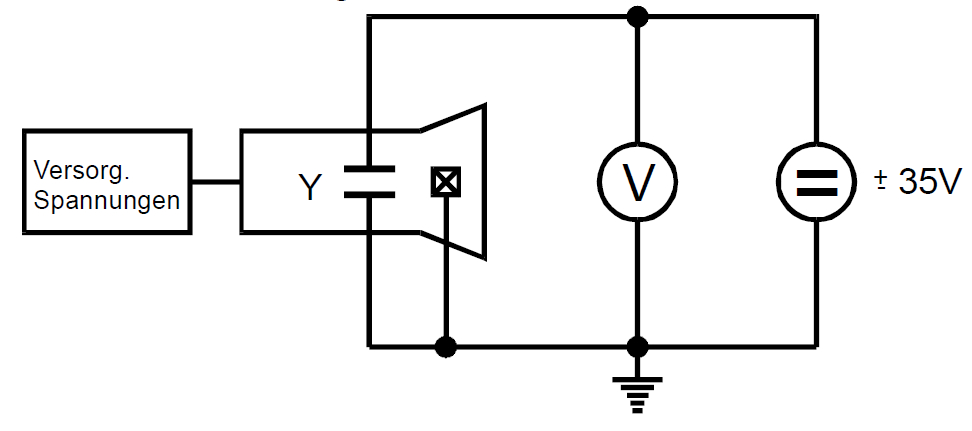
\includegraphics[width=\linewidth-70pt,height=\textheight-70pt,keepaspectratio]{content/images/Aufbau-E-Feld1.jpg}
\caption{Schaltung zur Messung der Verschiebung $D$ in Abhängigkeit von der Ablenkspannung $U_.d$ \cite{V501}.}
\label{fig:Aufbau-E1}
\end{figure}

\noindent Für den zweiten Versuchsteil im elektrischen Feld wird eine Schaltung gemäß Abbildung \ref{fig:Aufbau-E2} aufgebaut. Die Versorgungsspannung entspricht wieder der Beschleunigungsspannung $U_.B$. An den X-Ausgang des Ablenksystems der Kathodenstrahlröhre wird die Sägezahnspannung mit dem Frequenzzähler angeschlossen. Der Y-Ausgang wird an einen Sinusgenerator angeschlossen. Auch hier wird jeweils eine der Platten der Ablenksysteme geerdet.

\begin{figure}
\centering
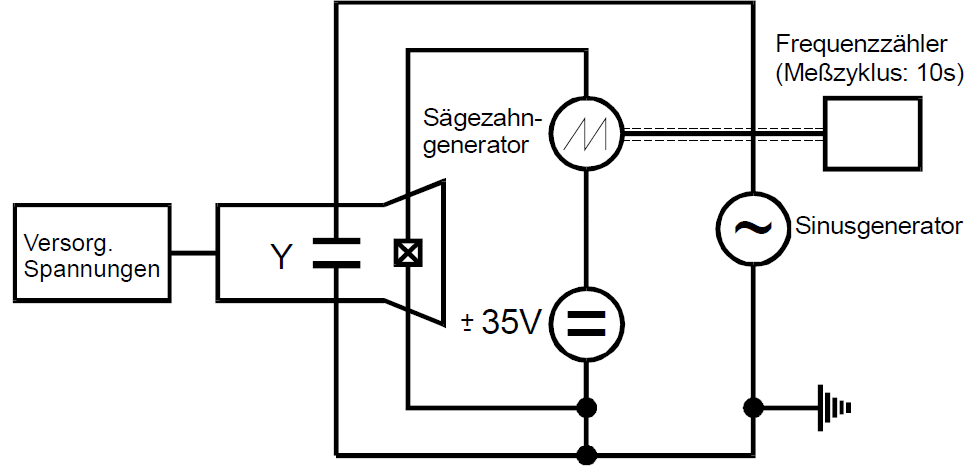
\includegraphics[width=\linewidth-70pt,height=\textheight-70pt,keepaspectratio]{content/images/Aufbau-E-Feld2.jpg}
\caption{Schaltung des Kathodenstrahloszillographen \cite{V501}.}
\label{fig:Aufbau-E2}
\end{figure}

\noindent Für die Messungen im magnetischen Feld wird eine Kathodenstrahlröhre im Zentrum einer Helmholtzspule befestigt, sodass sie senkrecht zur Bewegungsrichtung der Elektronen von einem Magnetfeld durchdrungen wird. Die Helmholtzspule ist auf einem Drehtisch befestigt, sodass sie an dem Erdmagnetfeld ausgerichtet werden kann. Die Kathodenstrahlröhre ist wie in \ref{fig:Aufbau-E1} verkabelt. Die Helmholtzspule ist an einer Spannungsquelle angeschlossen, mit der die Stärke des Magnetfeldes reguliert werden kann.